\documentclass{article}

% for inserting images
\usepackage{graphicx}

% highlighting hyper links
\usepackage[colorlinks = true, citecolor = blue]{hyperref}

% package to adjust line spacing
\usepackage{setspace}

% package for setting the margins
\usepackage[margin = 1in]{geometry}

% indents the first paragraph in a section
\usepackage{indentfirst}

\title{DS 710 Final Project Executive Report}
\author{Sean Murphy}
\date{May 2024}

% for single spacing
\singlespacing

\begin{document}

\maketitle

\section{Motivations and Research Questions}


For this project, I analyzed data from eight tables in the Wikipedia article 
\href{https://en.wikipedia.org/wiki/List_of_world_records_in_athletics}{``List of world records in athletics"}, 
which contain current track and field world records broken down by gender, indoor versus outdoor events, and 
official versus unofficial records.  I will say more about the data itself and the process of obtaining it 
later.  

When examining the data set initially, several intriguing questions surfaced that I sought to address in this 
analysis.  I noticed that along with each record was an associated nation from which the athlete hailed.  
Oftentimes, these records (particularly the official records) are set at major world events like the Olympic 
Games and the World Championships in Athletics, at which nations compete with each other.  I wanted to get an 
idea for which nations tend to excel in track and field events in terms of the number of records they hold.  
Since I also know that this dominance can vary by event type, I wanted to examine the leading nations in each 
event category (sprinting, long distance, throwing, jumping, etc.) to see what the general trends have been.  

Since the data set also contains the dates the records were set, this provided a great opportunity to examine 
how long records tend to last in each event category, to examine the proportion of records lasting from each 
decade, and to zero in on trends for the longest lasting records overall.  Examining the length of time that 
records last by category can give an idea of whether some categories of events have more stable records, either 
because of there being fewer opportunities to break them or because they simply are so relatively excellent.

Finally, another interesting dimension to include in the analysis was the gender dimension.  The goal here 
would be to see whether the general trends for leading track and field nations and the longest lasting records 
by event category hold for both men's and women's events.  If not, this would be a good entry point to determine 
why there are variations in these trends.

\section{Data Collection Methods and Provenance}

As alluded to above, the data for this project was scraped from the Wikipedia article 
\href{https://en.wikipedia.org/wiki/List_of_world_records_in_athletics}{``List of world records in athletics"}.  
While there are 11 tables on this page, three of them are quite small and will be omitted; in total they contain 
four records, one of which is a mixed event and the other three of which are set under old javelin specifications.  
The other $8$ tables were scraped from the page and combined into one data frame, with the information on gender, 
setting (indoor vs. outdoor), and official records being included as added column fields.  The data was then 
cleaned to be used for analysis, as there were many irregularities in the date and athlete field formatting that 
had to be corrected.  Finally, additional fields were developed based on the event category, the duration the 
record lasted, and the decade in which the record was set, all of which proved useful in the subsequent analysis.

There are two licenses granting the  freedom to use Wikipedia content listed on the 
\href{https://en.wikipedia.org/wiki/Wikipedia:Copyrights}{``Wikipedia:Copyrights"} page.  The two licenses are 
the Creative Commons Attribution-ShareAlike $4.0$ International License and the GNU Free Documentation License.  
Copies of both licenses can be found at the hyperlink above, and more information can be found in the ``Data 
Provenance" document.

\section{Results}

\subsection{Dominant Track and Field Nations}

In order to examine the results I will proceed in the order I introduced the research questions above.  The first 
question concerned leading track and field nations in terms of their world record count.  Particularly, I was 
interested to find the nations with the highest world record counts, and then to examine national dominance by 
event category.  

In terms of the overall results, the United States is the clear leader with a remarkable $109$ records, followed 
by Kenya with $53$, Ethiopia with $31$, Russia with $23$, and Jamaica with $20$.  The dominance of Kenya, Ethiopia, 
and Jamaica are all particularly impressive given their relatively small population size.  As we will see later, 
national dominance certainly varies with the level of granularity at which track and field records are examined.  

To that end, I then proceeded to chart the top $5$ nations in terms of record count \textit{for each event category}, 
to see which nations tend to dominate in which kinds of events.  The plots are in Figure~\ref{fig:top_5}.  

The USA has the clear lead in six of the nine event categories: hurdles, relays, sprints, jumping, throwing, and 
multisport events.  Kenya and Ethiopia tend to dominate the pack in long distance and middle distance events, with 
Kenya having a whopping $40$ world records in long distance events.  Jamaica tends to do quite well in sprinting 
events, with $12$ world records currently held in that category.  Walking events are uniquely dominated by Russia 
with $9$ world records, followed by Italy with $6$.  The USA is conspicuously absent from the walking event leader 
board, while they are present in the top 5 nations of every other category.  Thus, we see that certain nations tend 
to excel in particular events, no doubt events for which their world-class athletes train with special emphasis.  
It would be fascinating to observe how this same chart would change over the course of the next century.  

% introduce the top five nations by category plots
\begin{figure}
    \centering
    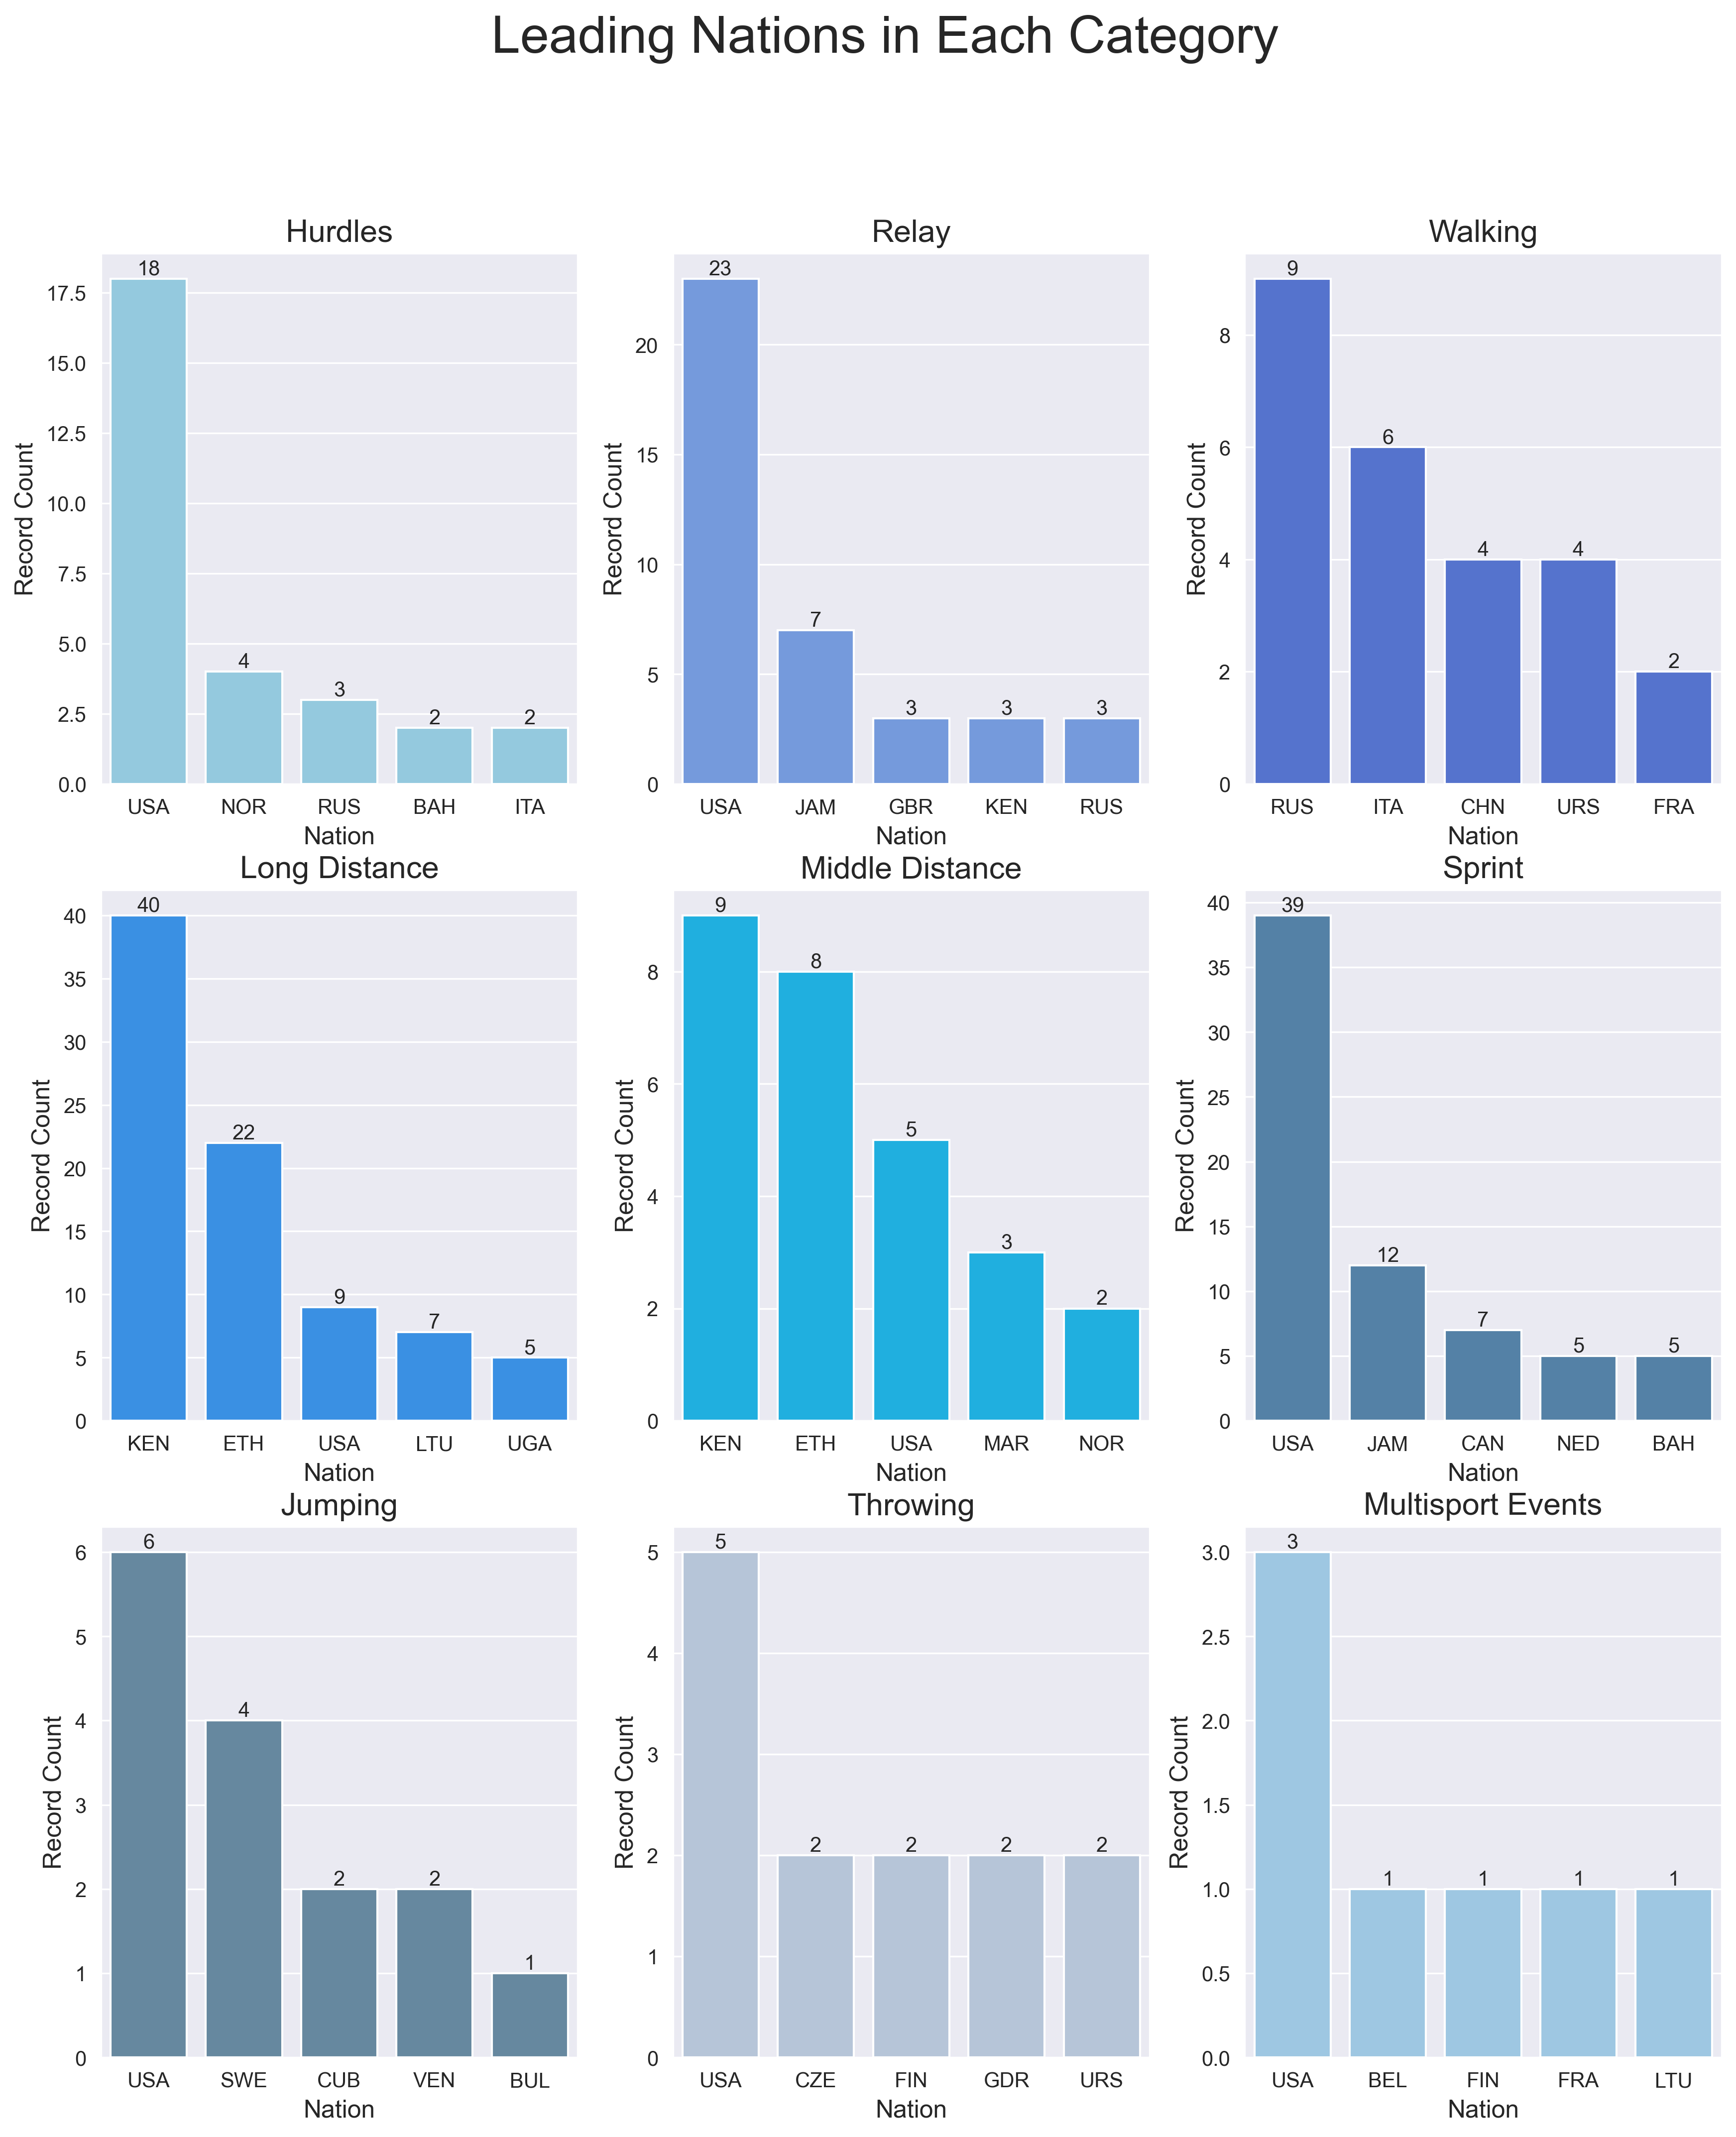
\includegraphics[scale = 0.5]{top_5_by_category.png}
    \caption{Top five nations by event category.}
    \label{fig:top_5}
\end{figure}

\subsection{Record Duration}

The next portion of the analysis was three-fold: to examine the proportion of existing records set in each decade, 
to look for trends in the longest lasting records, and to get an idea for how long records tend to last in each 
category.  

In answer to the first question, I calculated the proportion of the total records occupied by the records that fell 
within each decade.  In general, the majority of records now in existence (roughly $65\%$) were set in the twenty-first 
century.  It is somewhat surprising to me to note that almost one-third ($30.2\%$) of all records now in existence 
were set in the present decade, even though it is not yet halfway complete.  It is also fascinating to note on the 
other side of things that there are existing records dating as far back as the first decade of the twentieth century, 
the $1900s$.  The fact that this decade would even comprise a non-zero proportion of the total records is a marvel.  

Following this train of thought, I then proceeded to examine more carefully these longest lasting records.  In the 
data set, there are three records dating all the way back to the $1900s$ and one record dating back to the $1930s$.  
These are outliers that demand attention, since the next longest lasting record dates back only to the $1960s$.  As 
it turns out, each one of these records was set in a steeplechase event of varying distances.  The distances of 
$4,000$ m, $2,500$ m, $2,590$ m, and $3,460$ m represent steeplechase events which were historically held in the Olympics 
but are no longer, since the predominant steeplechase event is the $3,000$ m nowadays.  This explains why these records 
have lasted as long as they have, because they are seldom, if ever, officially contested.  

Finally, I wanted to get an idea of how long records tend to have lasted in each event category.  A quick look at the 
histogram in Figure~\ref{fig:hist} of the number of years that records have lasted reveals a strong positive skew to 
this metric, which indicates that the average duration will likely be slightly longer than the median duration for 
most categories.  And in fact, as we look at the plots in Figure~\ref{fig:avg_med}, which compares these two values 
for each category, we see that this pattern is mostly true.  

In this data set, sprinting records tend to have lasted the longest, with an average of just over $26$ years and a 
median of $28$ years.  The records that have lasted for the shortest period of time in the data set are the long 
distance records, with an average of just under $9$ years and a median of $4$ years.  

% introduce the histogram
\begin{figure}
    \centering
    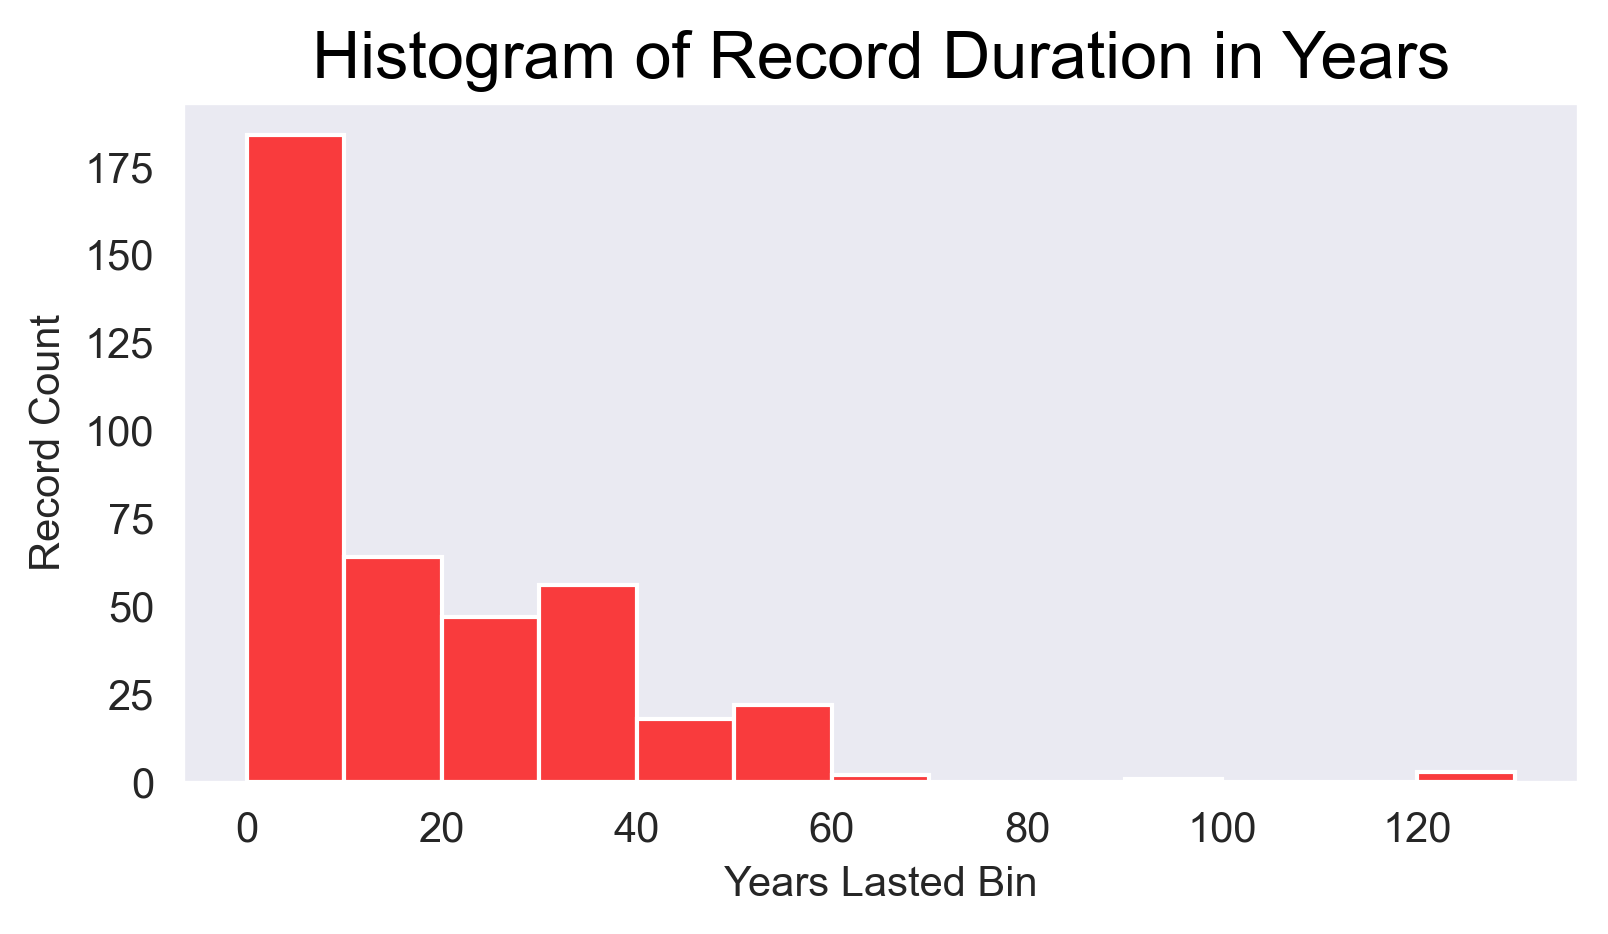
\includegraphics{years_lasted_histogram.png}
    \caption{Histogram of record duration in years.}
    \label{fig:hist}
\end{figure}

% introduce the average and median years lasted plots
\begin{figure}
    \centering
    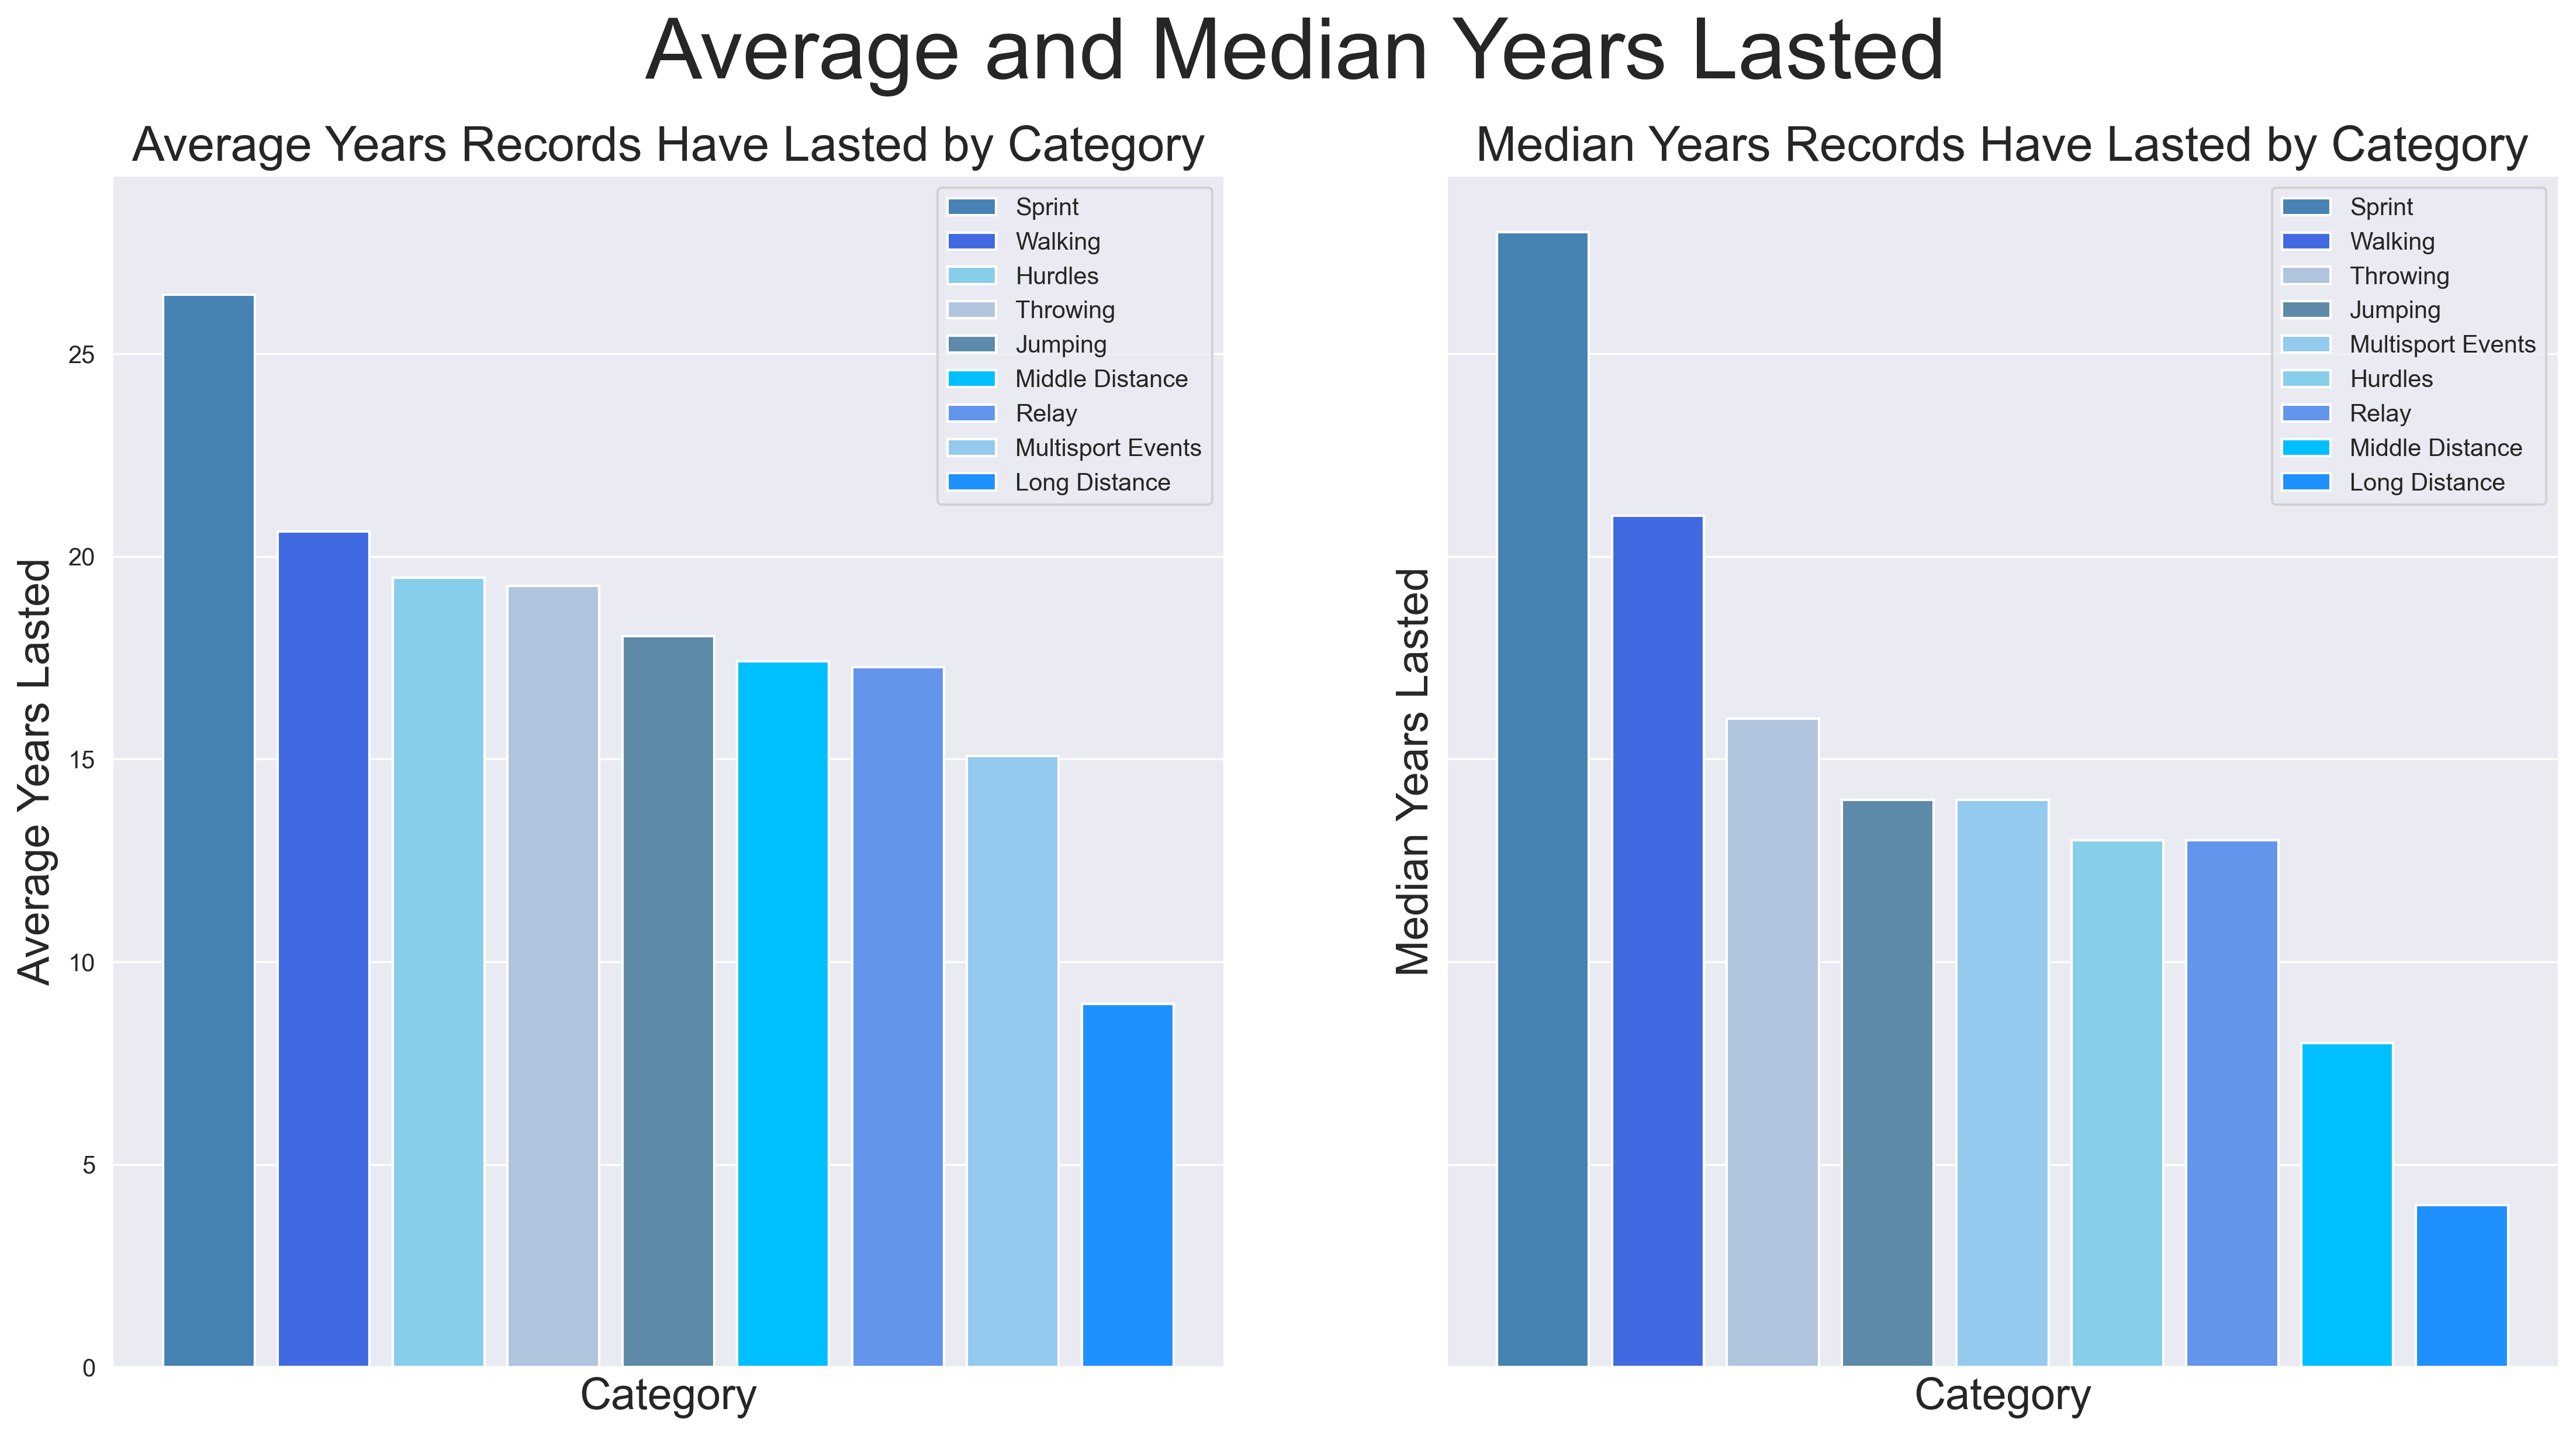
\includegraphics[scale = 0.4]{avg_and_med_years_lasted.png}
    \caption{Average and median years records have lasted in each event category.}
    \label{fig:avg_med}
\end{figure}

\subsection{Trends Along the Gender Dimension}

Finally, I wanted to examine whether the trends observed above tend to hold when they are analyzed separately for 
male versus female events.  With respect to the length of time that the records in the data set have lasted when 
broken down by event category, the trend does seem to hold regardless of the gender.  Sprinting events are the 
events that have lasted the longest, while long distance events are among those that have tended to last for the 
shortest period of time.  

With respect to overall national dominance in track and field events, however, there are a few notable differences 
between male and female events.  For men's events, the United States' dominance in terms of overall record count 
is very large.  The USA has more than triple the record count of the next highest nation.  For women's events, 
this dominance is not nearly as extreme.  The USA has only $8$ more records than its nearest competitor, Kenya.  
Moreover, for women's events, Ethiopia and Russia occupy the third and fourth positions in terms of record counts 
respectively, while they are much lower on the leader board in men's events.  Canada and Lithuania hold high 
positions on the leader board for men's events (fourth and fifth respectively), but neither of these nations are 
in the top ten for women's events.  In short, the amount of records held by each nation varies notably for men's 
events versus women's events.  

\section{Future Analysis Questions}

The above analysis, of course, is not exhaustive.  There is richness in the current data set that has not yet been 
explored, and there are also plenty of avenues where additional data would greatly broaden the scope of the analysis.  
I will discuss a few such avenues here.  

First, within the present data set, there is information on whether each record is official or unofficial.  There 
are also numerical measurements of the actual performance that was recorded.  For certain events the performance is 
measured in points, like a decathlon.  Other events, like races, are timed.  For other events, like jumps, the 
performance is measured in terms of distance.  It would be a fascinating portion of a future analysis to perform 
pairwise comparisons of performances for official versus unofficial events.  This 
would enable us to see which of the two tend to have the more impressive results.  

Another avenue of interest would be to assess record churn.  This would be the rate at which given records tend to 
be beaten within specific categories.  This present analysis was unable to include a portion on churn because the 
data set here does not contain historical record data; it only includes currently-standing records.  If such 
historical data were included, this would enable us to compare churn rates for different event categories.  
Additionally, depending upon the amount of additional data gathered, it could enable us to develop predictive 
models for which record types are likely to last for longer periods of time, and which records are likely to be 
beaten soon.  All of these considerations would greatly broaden the scope of the present analysis and would enhance 
the insights to be gleaned from examining track and field world record data.  

\end{document}